
%(BEGIN_QUESTION)
% Copyright 2007, Tony R. Kuphaldt, released under the Creative Commons Attribution License (v 1.0)
% This means you may do almost anything with this work of mine, so long as you give me proper credit

Explain the operation of this {\it cascade} temperature control system:

$$\includegraphics[width=15.5cm]{i01690x01.eps}$$

Cascade control systems (also called {\it two-element} control systems) have two control ``loops'' functioning: a {\it master} and a {\it slave} (also known as {\it primary} and {\it secondary}, respectively).  Identify the master (primary) and slave (secondary) loops in this temperature control system, and also determine which loop should be tuned {\it first} (and why!).

Also, identify the appropriate controller actions for each loop, assuming direct-acting transmitters and an air-to-open valve.  Annotate this diagram with ``+'' and ``$-$'' symbols showing the influences PV and SP have on each controller, and explain how these symbols help your analysis of the controllers' actions.

\vskip 20pt \vbox{\hrule \hbox{\strut \vrule{} {\bf Suggestions for Socratic discussion} \vrule} \hrule}

\begin{itemize}
\item{} A useful problem-solving strategy for determining necessary controller actions in a cascade control system is to replace the ISA-standard ``bubble'' symbols for controllers with triangular opamp symbols, complete with ``+'' and ``$-$'' symbols at the inputs.  One input of each ``opamp'' controller will be the PV, while the other input of each ``opamp'' controller will be the SP.  The inverting and noninverting inputs standard to all operational amplifiers helps remind you that the PV and SP inputs of a loop controller always have opposite effects on the output signal.
\item{} When tuning each loop controller (TIC, FIC), what should be done with the {\it other} controller?  Should the other controller be in automatic mode or manual mode, and why?
\item{} Suppose the control valve were switched from air-to-open to air-to-close.  Would {\it both} master and slave controller actions need to be reversed, or just one of the controllers?  If just one, which one?
\end{itemize}

\underbar{file i01690}
%(END_QUESTION)





%(BEGIN_ANSWER)

The temperature controller (TC) provides a ``remote'' setpoint to the flow controller (FC), which throttles the flow control valve (FV) to achieve the desired rate of steam flow.  

\begin{itemize}
\item{}Master (primary) = Reactor temperature
\item{}Slave (secondary) = Steam flow
\end{itemize} 

When tuning cascaded loops, you should {\it always} ensure the slave loop is well-tuned before attempting to tune the master loop.  I'll let you figure out why this is important!

\vskip 10pt

$$\includegraphics[width=15.5cm]{i01690x02.eps}$$

\vskip 10pt

\filbreak

A helpful strategy for identifying necessary master and slave controller actions in a cascade control system is to re-draw the controller ``bubbles'' as opamp symbols instead, complete with ``+'' and ``$-$'' labels for noninverting and inverting inputs, respectively.  Since all PID controllers have PV and SP inputs, and these inputs always have opposite effects on the output signal, the opamp conventions of ``+'' and ``$-$'' work very well to describe the action of any PID controller.  If the PV input on the opamp controller must be noninverting (``+'') in order to achieve loop stability, then that controller must be direct-acting.  If the PV input on the opamp controller must be inverting (``$-$'') in order to achieve loop stability, then that controller must be reverse-acting.  The following diagram shows how to use opamp symbols to represent controller actions in the same cascaded flow/temperature control system:

$$\includegraphics[width=15.5cm]{i01690x03.eps}$$

Note that it is always the {\it inputs} of a controller we label with ``+'' or ``$-$'' symbols, never the {\it output} of a controller.

%(END_ANSWER)





%(BEGIN_NOTES)

If the steam supply pressure changes for any reason, the flow controller will take immediate action to re-establish the proper steam flow rate {\it before} any effect is seen on the reactor temperature.  The practical advantage of having the flow control loop is to provide relative immunity to changes in steam header pressure.

The slave (secondary) loop is the one that ``takes orders'' from the master (primary) loop.  Since it is the steam flow controller that receives a setpoint from the temperature controller in this example, the FC is the slave and the TC is the master.

\vskip 10pt

Given an air-to-open control valve, both controllers need to be {\it reverse-acting}.

%INDEX% Control, strategies: cascade
%INDEX% Process: steam-heated reactor vessel (generic)

%(END_NOTES)


